\chapter{Quả cầu lửa, hệ quy chiếu và bốn-vectơ}

Chúng ta bắt đầu với một câu hỏi còn lại từ cuộc thảo luận về các va chạm năng lượng cao. Một va chạm của hai hạt nhân nặng tạo ra một đối tượng biến đổi dữ dội, chứ không phải một lỗ đen thiên văn yên ắng. Vậy thì mô tả va chạm đó bằng một chân trời có thể có nghĩa là gì? Câu trả lời dẫn qua một bức tranh năm chiều về vật chất ở chế độ ghép mạnh, một loạt câu hỏi thực tiễn về máy gia tốc, và cuối cùng quay trở lại hình học của thuyết tương đối hẹp. Đến cuối cùng, vận tốc và động lượng đã trở thành các bốn-vectơ, còn năng lượng đã đứng bên cạnh ba thành phần của động lượng.

\section{Một quả cầu lửa trong chiều không gian thứ năm}

\begin{classroomqa}
\audiencequestion{Đối tượng được tạo ra trong va chạm là không ổn định và thay đổi hình dạng. Làm sao một vật thể phức tạp như vậy lại có thể được gọi là lỗ đen?}
\lecturerresponse{Hãy hình dung một phương không gian thứ năm chạy giữa một cái sàn và một cái trần. Trọng lực theo phương đó kéo các kích thích về phía sàn. Va chạm đặt xuống đó một khối năng lượng nóng; khối ấy lan ra và đổi dạng, nhưng vẫn có thể có chân trời, nhiệt độ và entropy.}
\end{classroomqa}

Hãy tưởng tượng các hạt, hay hình tượng hơn là những sợi dây nhỏ, chuyển động trong thế giới năm chiều này. Những kích thích rơi xuống sàn xuất hiện trong bốn chiều dưới dạng các hadron: proton, neutron, meson và các đối tượng hợp thành mở rộng khác. Những kích thích gắn gần trần thì có vẻ cơ bản hơn. Vì thế, vị trí theo phương thẳng đứng là một cách hình học để mã hóa thang đo: sàn biểu diễn chế độ hadron ở khoảng cách lớn, còn trần biểu diễn các bậc tự do ở khoảng cách ngắn.

Khi hai hadron va chạm, hai đối tượng ở gần sàn đập vào nhau và làm bắn tóe ra một lượng năng lượng lớn. Kết quả không phải là một vật rắn. Nó là một khối nóng mang chân trời, một kiểu vũng năng lượng trong trường hấp dẫn năm chiều. Nó không phải là một lỗ đen thiên văn trong không gian bốn chiều thông thường, cũng không phải là một lỗ đen ở thang Planck gắn với trần. Nó là mô tả hấp dẫn của quả cầu lửa tương tác mạnh gần sàn.

Ở năng lượng cao, các hạt nhân tới bị co Lorentz thành những chiếc bánh dẹt mỏng. Chúng va chạm, gửi năng lượng của mình vào một vùng nhỏ và tạo ra một chất lưu lan ra và tiến tới cân bằng. Độ nhớt nhỏ của nó là một trong những đặc điểm gây ngạc nhiên của plasma quark--gluon. Trong mô tả năm chiều, cùng một sự tiến triển đó là sự thư giãn của một chân trời bị méo dạng.

\begin{figure}[H]
\centering
\includegraphics[width=0.82\textwidth]{lecture_05_figure_01.png}
\caption{Bức tranh sàn-và-trần của chiều thứ năm. Khối trung tâm mang chân trời lan dọc theo sàn sau va chạm.}
\lectureframe{00:04:22}
\end{figure}

Một chân trời không tồn tại mãi mãi. Bức xạ Hawking mang năng lượng đi, và trong mô tả bốn chiều, bức xạ ấy chính là cơn mưa các hadron thông thường xuất hiện từ va chạm. Hàng nghìn vệt ghi trong một sự kiện của đầu dò, theo ngôn ngữ này, là các hạt bị sôi tách ra khỏi lỗ đen đối ngẫu.

\subsection{Chiều phụ có thực không?}

\begin{classroomqa}
\audiencequestion{Chiều thứ năm có phải là một chiều không gian không, và đường được vẽ giữa sàn và trần có thực sự kéo dài theo phương đó không?}
\lecturerresponse{Có. Nó có tính không gian, và bề mặt được vẽ trong hình học năm chiều ấy là một chân trời. Việc ta gọi phương phụ đó là ``thực'' hay xem nó như một mô tả toán học tương đương là một câu hỏi sâu hơn.}
\end{classroomqa}

Điều hữu ích không phải là nói rằng hấp dẫn thay thế sắc động lực học lượng tử. Đúng hơn, hai ngôn ngữ có thể mô tả cùng một vật lý. Trong ngôn ngữ bốn chiều có một quả cầu lửa nóng gồm quark và gluon, không có trường hấp dẫn thông thường nào. Trong ngôn ngữ năm chiều có hấp dẫn và một chân trời. Nếu sự tương ứng là đúng, thì một phép tính QCD đúng nghĩa và phép tính hấp dẫn đối ngẫu phải cho cùng kết quả ở mọi nơi mà cả hai đều có thể thực hiện được.

\begin{classroomqa}
\audiencequestion{QCD không có hấp dẫn cũng không có chân trời. Bức tranh lỗ đen có đang thêm vào vật lý mới không, hay nó chỉ mô tả lại quả cầu lửa?}
\lecturerresponse{Trong bốn chiều, đó là một plasma quark và gluon; trong hiện thân năm chiều, nó có một mô tả hấp dẫn với một chân trời. Lợi thế nằm ở tính toán. QCD ở chế độ ghép mạnh cực kỳ khó, trong khi một số tính chất của chân trời---đặc biệt là độ nhớt---lại tương đối dễ tính.}
\end{classroomqa}

Sự phân biệt giữa ``chiều thực'' và ``phép tương tự toán học'' không nhất thiết phải được giải quyết trước khi mô tả ấy trở nên hữu ích. Một cấu trúc có được một cách hiểu vật lý khi nó kết hợp với các biến khác thành một hệ quy luật đơn giản hơn, mạch lạc hơn. Tuy vậy, không nên nói quá: các ứng dụng của đối ngẫu chuẩn/hấp dẫn đối với plasma quark--gluon được quan sát chỉ là những mô hình của động lực học ghép mạnh, chứ không phải là bằng chứng rằng QCD trong thế giới thực có một đối ngẫu hấp dẫn chính xác đã biết.\editorialnote{Sự bảo lưu này làm rõ vị thế hiện nay của ứng dụng QCD; nó không làm thay đổi cơ chế năm chiều được phát triển ở đây.}

\section{Vì sao máy va chạm cho hai chùm hạt va nhau}

Những câu hỏi bây giờ trở nên thực tiễn. Vì sao dùng hai chùm đang chuyển động thay vì một chùm đơn và một bia đứng yên? Vì sao máy gia tốc tròn lại lớn đến vậy? Vì sao electron và proton được xử lý khác nhau? Tất cả những câu hỏi ấy đều là những câu hỏi về năng lượng tương đối tính.

\begin{classroomqa}
\audiencequestion{Vì sao cho hai chùm va chạm nhau thay vì bắn một chùm năng lượng cao vào một bia đứng yên?}
\lecturerresponse{Điều tạo ra hạt mới là năng lượng sẵn có trong hệ quy chiếu khối tâm. Hai chùm tương đối tính bằng nhau và ngược chiều có tổng động lượng bằng không, nên về cơ bản hầu như toàn bộ năng lượng của chúng đều sẵn cho va chạm. Một bia cố định buộc phần lớn năng lượng của chùm tới phải còn lại dưới dạng chuyển động của khối tâm.}
\end{classroomqa}

Đối với hai hạt siêu tương đối tính có động lượng ngược chiều với độ lớn \(p\), ước lượng ở mức bài giảng trong các đơn vị \(c=1\) là
\begin{equation}
E_{\mathrm{cm}}^{\mathrm{collider}}\simeq 2p.
\end{equation}
Ước lượng tương ứng cho trường hợp bia cố định chỉ tăng theo căn bậc hai của động lượng chùm,
\begin{equation}
E_{\mathrm{cm}}^{\mathrm{fixed}}\sim \sqrt{mp}.
\end{equation}
Điều cốt yếu là quy luật tỉ lệ, chứ không phải hệ số số học đã được lược bỏ: gấp đôi năng lượng chùm thì gấp đôi năng lượng va chạm của collider, nhưng năng lượng khối tâm của cấu hình bia cố định chỉ tăng theo căn bậc hai.

Phép tính bất biến làm cho phép so sánh trở nên chính xác. Nếu \(P_1\) và \(P_2\) là các bốn-động lượng tới, thì
\begin{equation}
s=(P_1+P_2)^2,
\qquad E_{\mathrm{cm}}=\sqrt{s}.
\end{equation}
Đối với hai chùm ngược chiều có cùng năng lượng \(E\), các động lượng không gian triệt tiêu nhau và \(\sqrt{s}=2E\). Đối với một hạt bắn tới có năng lượng \(E\gg m\) đập vào một bia cùng khối lượng đang đứng yên,
\begin{equation}
s=2m^2+2mE,
\qquad
\sqrt{s}\simeq \sqrt{2mE}
\qquad (c=1).
\end{equation}
Suy dẫn ngắn gọn bằng bất biến này cung cấp hệ số đã bị lược bỏ trong ước lượng bằng lời.\editorialnote{Phần suy dẫn được đưa vào để lập luận về quy luật tỉ lệ trong bài giảng có thể được tái lập.}

\begin{classroomqa}
\audiencequestion{Có lý do cơ bản nào khiến một máy gia tốc tròn phải lớn đến vậy không? Có thể chỉ cho cùng một chùm đó lưu thông qua một máy nhỏ hơn nhiều vòng hơn không?}
\lecturerresponse{Trường và vật liệu đặt ra các giới hạn. Một hạt chỉ nhận được một độ tăng năng lượng hữu hạn trên mỗi mét, nên một máy năng lượng cao hơn cần một chiều dài gia tốc hiệu dụng lớn hơn. Một vòng tròn chật hơn cũng đòi hỏi gia tốc ngang lớn hơn, và một điện tích bị gia tốc thì bức xạ. Nếu vòng quá nhỏ, chùm sẽ bức xạ năng lượng nhanh ngang với tốc độ máy cung cấp nó.}
\end{classroomqa}

Quan hệ bẻ cong xấp xỉ là
\begin{equation}
p=qBR,
\end{equation}
nên với từ trường \(B\) cố định, động lượng \(p\) lớn hơn đòi hỏi bán kính \(R\) lớn hơn. Các hốc cộng hưởng tần số vô tuyến thực hiện công làm tăng năng lượng chùm; còn nam châm bẻ cong và hội tụ chùm. Bài học tổng quát vẫn là điều đã nói trên bảng: cường độ trường và tổn hao bức xạ ngăn chúng ta nén một máy gia tốc có năng lượng tùy ý lớn vào một vòng nhỏ.

Chuyển động tròn có gia tốc ngay cả khi tốc độ không đổi vì vận tốc đổi hướng. Một điện tích bị gia tốc phát ra bức xạ synchrotron. Máy gia tốc thẳng tránh được tổn hao do bẻ cong liên tục, mặc dù bản thân các cú đẩy gia tốc ngắn ấy theo nghĩa đen không phải là hoàn toàn không bức xạ. Máy tròn chấp nhận cái giá của sự bẻ cong để đổi lấy việc tái sử dụng cùng một thiết bị trên mỗi vòng quỹ đạo.

\begin{classroomqa}
\audiencequestion{Vì sao electron gắn với máy gia tốc thẳng ở SLAC, trong khi các máy va chạm tròn năng lượng cao lại dùng proton hoặc các hadron khác?}
\lecturerresponse{Electron nhẹ hơn rất nhiều. Ở cùng một năng lượng cao, hệ số Lorentz của chúng lớn hơn nhiều, và gia tốc tròn khiến chúng bức xạ mạnh hơn hẳn. Các proton nặng hơn có thể quay vòng lặp đi lặp lại, nhận thêm năng lượng ở mỗi lần đi qua, trước khi tổn hao synchrotron trở nên không thể chấp nhận được.}
\end{classroomqa}

Với năng lượng và bán kính vòng cố định, công suất bức xạ phụ thuộc rất dốc vào khối lượng hạt,
\begin{equation}
P_{\mathrm{sync}}\propto \frac{E^4}{m^4R^2}.
\end{equation}
Đó là vì sao sự khác biệt electron--proton sắc nét hơn nhiều so với điều mà cụm từ ``hạt nhẹ hơn chuyển động nhanh hơn'' có thể gợi ra: cả hai chùm đều có thể đã cực kỳ gần \(c\), nhưng hệ số Lorentz và tổn hao bức xạ của chúng rất khác nhau.\editorialnote{Quan hệ bẻ cong và quy luật tỉ lệ synchrotron làm cho lập luận định tính về máy gia tốc trong bài giảng trở nên chính xác; chúng đã không được triển khai trên bảng.}

\begin{classroomqa}
\audiencequestion{Vì sao không gia tốc hadron trên một đường thẳng luôn?}
\lecturerresponse{Có thể. Khó khăn nằm ở chiều dài. Trong một vòng, cùng một hạt đi qua các cấu trúc gia tốc nhiều lần; một máy hadron thẳng tương đương sẽ phải dài khổng lồ. Giải pháp thỏa hiệp hữu ích là một vòng lớn, đủ lớn để bức xạ proton vẫn còn chấp nhận được.}
\end{classroomqa}

Những câu hỏi về máy gia tốc này cho thấy chính xác vì sao các quy tắc Newton là không đủ. Bây giờ ta quay lại thuyết tương đối hẹp và xây dựng ngôn ngữ khiến những so sánh như vậy trở nên có hệ thống.

\section{Ga-ra và chiếc limousine}

Hãy xét một ga-ra dài khoảng 12 foot và một chiếc limousine kéo dài khoảng 20 foot. Người lái tăng tốc cho đến khi chiếc limousine bị co Lorentz, hy vọng nó sẽ lọt vào. Trong hệ quy chiếu của ga-ra, chiếc limousine đang chuyển động ngắn hơn, nên điều đó có vẻ khả thi. Tuy nhiên, trong hệ quy chiếu của limousine, ga-ra đang chuyển động ngắn hơn, nên điều đó có vẻ bất khả thi. Toàn bộ chiếc limousine có thể nằm trong ga-ra hay không?

Mở cả hai cửa để việc va vào tường không làm ta phân tâm. Nói rằng chiếc limousine ở trong có nghĩa là đầu trước và đầu sau của nó đều ở trong \emph{đồng thời}. Từ cuối cùng đó chứa trọn toàn bộ câu đố.

Hãy vẽ một giản đồ không-thời gian với \(t\) thẳng đứng và \(x\) nằm ngang. Các tia sáng tạo thành nón ánh sáng \(45^\circ\) trong đơn vị \(c=1\). Ga-ra đứng yên, nên các đường thế giới của hai cánh cửa là thẳng đứng. Đầu trước và đầu sau của chiếc limousine vạch ra hai đường thế giới nghiêng song song. Trục \(t'\) của hệ chuyển động nghiêng về phía nón ánh sáng, và các đường đồng thời của nó song song với trục \(x'\) đã nghiêng.

\begin{figure}[H]
\centering
\includegraphics[width=0.82\textwidth]{lecture_05_figure_02.png}
\caption{Giản đồ không-thời gian ga-ra--limousine hoàn chỉnh. Các đường thẳng đứng giới hạn ga-ra; các đường nghiêng vạch ra hai đầu của chiếc limousine. Các lát cắt ngang và nghiêng biểu diễn các lát đồng thời khác nhau của hai hệ quy chiếu.}
\lectureframe{00:31:05}
\end{figure}

Trong hệ quy chiếu của ga-ra, một đường ngang có thể cắt cả hai đường thế giới của limousine ở giữa hai đường thế giới của ga-ra. Ở thời điểm đó theo ga-ra, phần sau đã vào và phần trước vẫn chưa ra. Chiếc limousine đã co nằm hoàn toàn bên trong.

Trong hệ quy chiếu của limousine, các sự kiện đồng thời liên quan nằm trên một đường nghiêng. Hãy vẽ một đường như vậy đi qua sự kiện tại đó phần sau đi vào. Nó cắt đường thế giới của phần trước sau khi đầu trước đã đi qua cửa xa rồi. Theo tính đồng thời riêng của nó, chiếc limousine không bao giờ nằm hoàn toàn bên trong. Cả hai phát biểu đều đúng vì chúng so sánh những cặp sự kiện khác nhau.

\begin{classroomqa}
\audiencequestion{Hai đường thế giới màu xanh lá và đoạn nằm ngang giữa chúng có tạo thành một hình bình hành không? Đoạn màu đen đó có phải là chiều dài của chiếc xe không?}
\lecturerresponse{Đoạn nằm ngang là chiều dài bị co Lorentz, vì hai đầu mút của nó là đồng thời trong hệ quy chiếu của ga-ra. Độ dài riêng được lấy từ các đầu mút đồng thời trong hệ quy chiếu của xe limousine, trên một đường thẳng song song với \(x'\). Hai phép đo dùng những lát cắt khác nhau qua cùng một cặp đường thế giới.}
\end{classroomqa}

Nếu \(L_0\) là độ dài riêng, thì lát cắt nằm ngang trong hệ quy chiếu ga-ra có độ dài
\begin{equation}
L=\frac{L_0}{\gamma},
\qquad
\gamma=\frac{1}{\sqrt{1-v^2/c^2}}.
\end{equation}
Chỉ riêng công thức thì không giải quyết được nghịch lý. Hình vẽ làm được điều đó, vì nó cho thấy những sự kiện nào đã được đem so sánh. Bất cứ khi nào một bài toán đố về thuyết tương đối dường như cho ra hai đáp án không tương thích, hãy tìm xem từ ``đồng thời'' có đang được dùng ngầm hay không.

\section{Bốn tọa độ và hai vị trí của chỉ số}

Để chuyển từ các nghịch lý sang các định luật chuyển động, ta cần một ký hiệu ghi nhớ hình học. Gom các tọa độ lại thành
\begin{equation}
(X^1,X^2,X^3,X^0)=(x,y,z,t),
\qquad X^\mu=(x,y,z,t),
\end{equation}
trong đó \(\mu\) chạy qua \(1,2,3,0\). Thứ tự này đặt thời gian ở cuối trên trang giấy dù chỉ số của nó là \(0\), phù hợp với quy ước được dùng trên bảng.

\begin{classroomqa}
\audiencequestion{Chúng ta có đang đặt \(c=1\) không? Nếu khôi phục các đơn vị thông thường, thì tọa độ thời gian có phải là \(ct\) không?}
\lecturerresponse{Có. Ta đặt \(c=1\) khi triển khai phần hình học và đưa các thừa số \(c\) trở lại khi cần xét thứ nguyên hoặc giới hạn phi tương đối tính. Với đơn vị chiều dài thông thường, tọa độ thời gian là \(ct\).}
\end{classroomqa}

Cùng một vectơ có thể được viết với chỉ số dưới. Với quy ước dấu dùng ở đây,
\begin{equation}
X_\mu=(-x,-y,-z,t).
\end{equation}
Vì vậy, hạ một chỉ số sẽ đảo dấu ba thành phần không gian và giữ nguyên thành phần thời gian. Ví dụ,
\begin{equation}
X^\mu=(3,2,4,10)
\quad\Longrightarrow\quad
X_\mu=(-3,-2,-4,10).
\end{equation}
Đây không phải là hai điểm không-thời gian; chúng là hai dạng thành phần của cùng một đối tượng hình học.

\begin{classroomqa}
\audiencequestion{Những thành phần nào là hiệp biến và phản biến, và các nhãn ấy là chỉ số trên hay chỉ số dưới?}
\lecturerresponse{Các thành phần mang chỉ số trên là phản biến; các thành phần mang chỉ số dưới là hiệp biến. Một mẹo ghi nhớ hữu ích ngay trong lớp là ``co thì thấp, contra thì cao.'' Các nhà vật lý thường đơn giản gọi chúng là chỉ số trên và chỉ số dưới.}
\end{classroomqa}

Ký hiệu này phát huy tác dụng trong phép co bất biến
\begin{equation}
X_\mu X^\mu=t^2-x^2-y^2-z^2.
\label{eq:l5-interval}
\end{equation}
Dưới dạng vi phân, ta có
\begin{equation}
d\tau^2=dt^2-dx^2-dy^2-dz^2
\qquad (c=1).
\label{eq:l5-proper-time}
\end{equation}
Đối với chuyển động kiểu thời gian, \(d\tau\) là thời gian mà một đồng hồ chuyển động dọc theo đường thế giới ghi lại.

Mỗi khi cùng một chỉ số xuất hiện một lần ở trên và một lần ở dưới, ta ngầm hiểu là phải lấy tổng. Quy ước Einstein biến
\begin{equation}
\sum_{\mu}X_\mu X^\mu
\end{equation}
thành biểu thức ngắn hơn trong phương trình~\eqref{eq:l5-interval}. Đây không chỉ đơn thuần là tiết kiệm ký hiệu. Nó ngăn không cho các dấu xen kẽ của hình học Minkowski phải được viết lại bằng tay trong mọi phương trình.

\begin{classroomqa}
\audiencequestion{Có phải \(\tau\) là ký hiệu chuẩn cho thời gian riêng không?}
\lecturerresponse{Có. Ký hiệu \(s\) đôi khi cũng được dùng, nhưng \(\tau\) là một lựa chọn chuẩn cho thời gian riêng.}
\end{classroomqa}

\section{Phép quay như một đối xứng dễ xử lý}

Một phép boost Lorentz trộn lẫn không gian và thời gian. Trước khi khảo sát ma trận đó, hãy xét phép toán quen thuộc hơn là quay các trục không gian. Nếu chuyển động tương đối hướng theo một phương bất kỳ, ta có thể quay các trục cho đến khi phương đó trở thành trục \(x\) mới rồi áp dụng phép boost đã biết. Vì vậy, các phép quay là một phần của cách xây dựng, chứ không phải một đường vòng mang tính trang trí.

Đối với phép quay một góc \(\theta\) quanh trục \(z\),
\begin{align}
x'&=x\cos\theta+y\sin\theta,\nonumber\\
y'&=-x\sin\theta+y\cos\theta,\label{eq:l5-rotation}\\
z'&=z.\nonumber
\end{align}
Khi \(\theta=0\), các phương trình này cho lại \(x'=x\) và \(y'=y\); khi \(\theta=\pi/2\), chúng hoán đổi hai trục với các dấu như dự kiến.

Phép biến đổi này bảo toàn khoảng cách Euclid. Viết
\(c_\theta=\cos\theta\) và \(s_\theta=\sin\theta\),
\begin{align}
x'^2+y'^2
&=(xc_\theta+ys_\theta)^2+(-xs_\theta+yc_\theta)^2\nonumber\\
&=x^2(c_\theta^2+s_\theta^2)
  +y^2(s_\theta^2+c_\theta^2)\nonumber\\
&\quad+2xyc_\theta s_\theta-2xyc_\theta s_\theta\nonumber\\
&=x^2+y^2.
\end{align}
Các hạng chéo triệt tiêu nhau và \(c_\theta^2+s_\theta^2=1\). Vì \(z'=z\),
độ dài đầy đủ \(x^2+y^2+z^2\) là bất biến.

Cũng các phương trình ấy có thể gộp thành một phương trình ma trận:
\begin{equation}
\begin{pmatrix}x'\\y'\\z'\end{pmatrix}
=
\underbrace{\begin{pmatrix}
\cos\theta&\sin\theta&0\\
-\sin\theta&\cos\theta&0\\
0&0&1
\end{pmatrix}}_{M}
\begin{pmatrix}x\\y\\z\end{pmatrix}.
\label{eq:l5-rotation-matrix}
\end{equation}
Theo ký hiệu chỉ số,
\begin{equation}
x'^i=M^i{}_{j}x^j,
\qquad i,j=1,2,3.
\end{equation}

\begin{figure}[H]
\centering
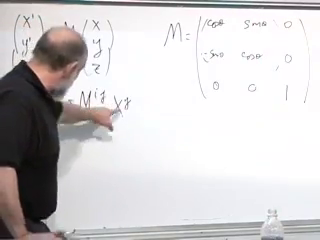
\includegraphics[width=0.82\textwidth]{lecture_05_figure_03.png}
\caption{Phép quay không gian được viết cả dưới dạng phương trình ma trận lẫn dưới ký hiệu chỉ số.}
\lectureframe{01:00:40}
\end{figure}

\section{Ma trận Lorentz và vận tốc hợp thành}

Đối với chuyển động dọc theo \(x\), phép biến đổi Lorentz trong đơn vị \(c=1\) là
\begin{align}
x'&=\gamma_v(x-vt), & y'&=y,\nonumber\\
z'&=z, & t'&=\gamma_v(t-vx),
\end{align}
trong đó
\begin{equation}
\gamma_v=\frac{1}{\sqrt{1-v^2}}.
\end{equation}
Với thứ tự thành phần \((x,y,z,t)\), điều này trở thành
\begin{equation}
\begin{pmatrix}x'\\y'\\z'\\t'\end{pmatrix}
=
\begin{pmatrix}
\gamma_v&0&0&-\gamma_vv\\
0&1&0&0\\
0&0&1&0\\
-\gamma_vv&0&0&\gamma_v
\end{pmatrix}
\begin{pmatrix}x\\y\\z\\t\end{pmatrix}.
\label{eq:l5-lorentz-matrix}
\end{equation}

\begin{figure}[H]
\centering
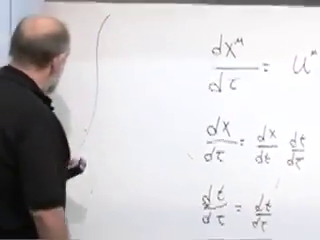
\includegraphics[width=0.82\textwidth]{lecture_05_figure_04.png}
\caption{Ma trận Lorentz \(4\times4\). Chỉ có các thành phần \(x\) và \(t\) trộn lẫn với nhau; \(y\) và \(z\) giữ nguyên.}
\lectureframe{01:04:40}
\end{figure}

Phép nhân ma trận giờ đây trả lời một câu hỏi vật lý. Giả sử một quan sát viên chuyển động với vận tốc \(v\) so với chúng ta và một người thứ ba chuyển động với vận tốc \(u\) so với quan sát viên đó, tất cả đều dọc theo cùng một trục. Động học Newton sẽ cho \(w=u+v\), điều này sẽ cho phép hai vận tốc \(3c/4\) hợp lại thành \(3c/2\). Thuyết tương đối phải cho một quy tắc khác.

Phần tác dụng của phép boost là ma trận \(2\times2\)
\begin{equation}
B(v)=\gamma_v
\begin{pmatrix}1&-v\\-v&1\end{pmatrix}.
\end{equation}
Ghép hai phép boost lại cho
\begin{align}
B(u)B(v)
&=\gamma_u\gamma_v
\begin{pmatrix}1&-u\\-u&1\end{pmatrix}
\begin{pmatrix}1&-v\\-v&1\end{pmatrix}\nonumber\\
&=\gamma_u\gamma_v
\begin{pmatrix}
1+uv&-(u+v)\\
-(u+v)&1+uv
\end{pmatrix}.
\label{eq:l5-composed-boost}
\end{align}
Tỷ số giữa một phần tử ngoài đường chéo và một phần tử trên đường chéo xác định vận tốc của phép boost kết quả:
\begin{equation}
w=\frac{u+v}{1+uv}
\qquad(c=1).
\end{equation}
Khôi phục thứ nguyên,
\begin{equation}
w=\frac{u+v}{1+uv/c^2}.
\label{eq:l5-velocity-addition}
\end{equation}

\begin{figure}[H]
\centering
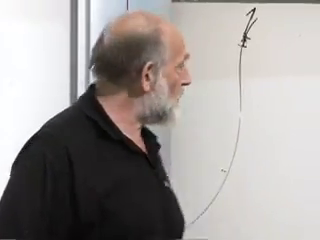
\includegraphics[width=0.82\textwidth]{lecture_05_figure_05.png}
\caption{Ma trận của phép boost hợp thành và vận tốc
\(w=(u+v)/(1+uv)\) trong đơn vị tự nhiên.}
\lectureframe{01:15:35}
\end{figure}

Nếu \(u\) và \(v\) đều gần \(c\), thì tử số tiến tới \(2c\) còn mẫu số tiến tới \(2\), nên \(w\) tiến tới \(c\), chứ không phải \(2c\). Nói tổng quát hơn, phương trình~\eqref{eq:l5-velocity-addition} ánh xạ các đầu vào dưới tốc độ ánh sáng thành một kết quả cũng dưới tốc độ ánh sáng. Phép nhân ma trận đã tự động mã hóa giới hạn tốc độ.

\section{Bốn-vectơ và sự thất bại của vận tốc thông thường}

Một bốn-vectơ là bất kỳ đối tượng nào có bốn thành phần biến đổi dưới phép quay và boost Lorentz theo cùng cách như các tọa độ không-thời gian. Nếu \(V^\mu\) là một bốn-vectơ, thì với quy ước dấu của chúng ta
\begin{equation}
V_\mu=(-V^1,-V^2,-V^3,V^0),
\end{equation}
và chuẩn bất biến của nó là
\begin{equation}
V_\mu V^\mu=(V^0)^2-(V^1)^2-(V^2)^2-(V^3)^2.
\end{equation}
Đối với hai bốn-vectơ \(V^\mu\) và \(W^\mu\), phép co
\begin{equation}
W_\mu V^\mu
=W^0V^0-W^1V^1-W^2V^2-W^3V^3
\end{equation}
cũng bất biến. Các thành phần thay đổi giữa các hệ quy chiếu; phép co thì không.

Vận tốc thông thường chỉ có ba thành phần,
\begin{equation}
\mathbf v=\left(\frac{dx}{dt},\frac{dy}{dt},\frac{dz}{dt}\right).
\end{equation}
Gắn thêm \(dt/dt=1\) không biến nó thành một bốn-vectơ hữu ích. Thành phần thứ tư sẽ là tầm thường, và đối tượng thu được sẽ không biến đổi tuyến tính dưới các phép biến đổi Lorentz. Thời gian tọa độ \(t\) thay đổi từ hệ quy chiếu này sang hệ quy chiếu khác, nên việc lấy đạo hàm theo \(t\) phá hỏng quy luật biến đổi mong muốn.

Thời gian riêng cung cấp cách khắc phục. Dọc theo một đường thế giới, định nghĩa
\begin{equation}
u^\mu=\frac{dX^\mu}{d\tau}.
\label{eq:l5-four-velocity}
\end{equation}
Vi phân \(dX^\mu\) là một bốn-vectơ và \(d\tau\) là bất biến, nên tỷ số của chúng là một bốn-vectơ. Tính từ ``riêng'' nói tới chiếc đồng hồ ở mẫu số.

Quy tắc dây chuyền liên hệ đối tượng này với vận tốc thông thường:
\begin{equation}
\frac{dx}{d\tau}=\frac{dx}{dt}\frac{dt}{d\tau},
\end{equation}
và tương tự cho \(y\) và \(z\). Từ phương trình~\eqref{eq:l5-proper-time},
\begin{align}
\left(\frac{d\tau}{dt}\right)^2
&=1-\left(\frac{dx}{dt}\right)^2
    -\left(\frac{dy}{dt}\right)^2
    -\left(\frac{dz}{dt}\right)^2\nonumber\\
&=1-v^2
\qquad(c=1),
\end{align}
và do đó
\begin{equation}
\frac{dt}{d\tau}=\gamma_v=\frac{1}{\sqrt{1-v^2}}.
\end{equation}
Bốn thành phần là
\begin{equation}
u^i=\gamma_v v^i,
\qquad
u^0=\gamma_v
\qquad(c=1).
\label{eq:l5-four-velocity-components}
\end{equation}
Ở tốc độ thấp, \(u^i\simeq v^i\) và \(u^0\simeq1\). Gần tốc độ ánh sáng,
\(\gamma_v\) tăng không bị chặn và vận tốc riêng khác biệt rõ rệt với vận tốc thông thường.

\begin{figure}[H]
\centering
\includegraphics[width=0.82\textwidth]{lecture_05_figure_06.png}
\caption{Bốn thành phần của vận tốc riêng được biểu diễn qua vận tốc thông thường và hệ số Lorentz.}
\lectureframe{01:34:40}
\end{figure}

Khôi phục các đơn vị thông thường và dùng \(X^0=ct\), ta được dạng chuẩn
\begin{equation}
U^\mu=(\gamma_v\mathbf v,\gamma_v c)
\end{equation}
trong thứ tự đặt các thành phần không gian trước được dùng ở đây. Chuẩn bất biến của nó là
\begin{equation}
U_\mu U^\mu=c^2.
\end{equation}
Vì vậy, mọi hạt có khối lượng đều có một bốn-vận tốc với cùng độ lớn bất biến, mặc dù vận tốc không gian của nó phụ thuộc vào hệ quy chiếu.

\section{Tiếp tuyến của một đường thế giới}

Có một mô hình Euclid quen thuộc cho phương trình~\eqref{eq:l5-four-velocity}.
Dọc theo một đường cong trong không gian ba chiều thông thường,
\begin{equation}
ds^2=dx^2+dy^2+dz^2.
\end{equation}
Độ dời vi phân \((dx,dy,dz)\) hướng dọc theo đường cong nhưng không phải là một vectơ đơn vị. Chia cho độ dài cung ta được
\begin{equation}
\mathbf T=
\left(\frac{dx}{ds},\frac{dy}{ds},\frac{dz}{ds}\right),
\qquad
\mathbf T\cdot\mathbf T=1.
\end{equation}
Cấu trúc tương đối tính cũng là cùng ý tưởng đó, với thời gian riêng thay cho độ dài cung Euclid. Vectơ \(u^\mu=dX^\mu/d\tau\) là tiếp tuyến của đường thế giới.

\begin{figure}[H]
\centering
\includegraphics[width=0.82\textwidth]{lecture_05_figure_07.png}
\caption{Cách dựng vectơ tiếp tuyến kiểu Euclid: chia độ dời vi phân cho phần tử độ dài cung \(ds\). Thời gian riêng đóng vai trò tương tự dọc theo một đường thế giới kiểu thời gian.}
\lectureframe{01:39:30}
\end{figure}

\begin{classroomqa}
\audiencequestion{Nếu \(c=1\), thì thời gian riêng và khoảng cách riêng có phải là như nhau không?}
\lecturerresponse{Đặt \(c=1\) khiến thời gian và khoảng cách có cùng đơn vị; điều đó không xóa đi các dấu trừ của hình học không-thời gian. Trong phép tương tự Euclid, \(s\) là khoảng cách thông thường đo dọc theo một đường cong không gian. Dọc theo một đường thế giới kiểu thời gian, \(\tau\) là khoảng thời gian trôi qua do đồng hồ đo được. Các cách dựng là tương tự nhau, nhưng các hình học thì khác nhau.}
\end{classroomqa}

Lấy đạo hàm thêm một lần nữa định nghĩa gia tốc riêng,
\begin{equation}
a^\mu=\frac{du^\mu}{d\tau}.
\end{equation}
Đây là đại lượng phải thay thế \(d^2\mathbf x/dt^2\) khi định luật II Newton được tương đối tính hóa. Vì \(u_\mu u^\mu\) là hằng số,
\begin{equation}
\frac{d}{d\tau}(u_\mu u^\mu)=2u_\mu a^\mu=0,
\end{equation}
nên bốn-gia tốc trực giao theo Minkowski với bốn-vận tốc.\editorialnote{Tính trực giao này suy ra ngay từ chuẩn bất biến và được đưa vào như hệ quả toán học tiếp theo của định nghĩa.}

\section{Bốn-xung lượng và năng lượng}

Xung lượng là ví dụ cuối cùng của chúng ta vì nó được bảo toàn trong va chạm và phân rã. Hạt có một khối lượng nội tại cố định \(m\), thường được gọi là khối lượng nghỉ. Nó không biến thiên theo vận tốc. Xung lượng tương đối tính là khối lượng cố định ấy nhân với bốn-vận tốc:
\begin{equation}
p^\mu=mu^\mu.
\label{eq:l5-four-momentum}
\end{equation}
Trong đơn vị \(c=1\),
\begin{equation}
p^i=\gamma_v m v^i,
\qquad
p^0=\gamma_v m.
\end{equation}
Ở vận tốc nhỏ \(\gamma_v\simeq1\), nên các thành phần không gian thu về xung lượng Newton \(m\mathbf v\). Ở vận tốc cao, chúng tăng nhanh hơn \(m\mathbf v\).

Thành phần thời gian là năng lượng. Với các đơn vị thông thường và \(X^0=ct\),
\begin{equation}
P^\mu=(\mathbf p,E/c)
=(\gamma_v m\mathbf v,\gamma_v mc),
\end{equation}
và do đó
\begin{equation}
E=\gamma_v mc^2
=mc^2\left(1-\frac{v^2}{c^2}\right)^{-1/2}.
\label{eq:l5-relativistic-energy}
\end{equation}

Để khôi phục cơ học thông thường, hãy đặt
\(\epsilon=v^2/c^2\ll1\). Khai triển nhị thức cho
\begin{equation}
(1-\epsilon)^p=1-p\epsilon+O(\epsilon^2).
\end{equation}
Lấy \(p=-1/2\),
\begin{align}
E
&=mc^2\left(1-\frac{v^2}{c^2}\right)^{-1/2}\nonumber\\
&=mc^2\left[1+\frac12\frac{v^2}{c^2}
  +O\!\left(\frac{v^4}{c^4}\right)\right]\nonumber\\
&=mc^2+\frac12mv^2+O\!\left(\frac{mv^4}{c^2}\right).
\label{eq:l5-energy-expansion}
\end{align}

\begin{figure}[H]
\centering
\includegraphics[width=0.82\textwidth]{lecture_05_figure_08.png}
\caption{Khai triển vận tốc thấp của năng lượng tương đối tính, bộc lộ năng lượng nghỉ và động năng Newton.}
\lectureframe{01:51:30}
\end{figure}

Số hạng thứ nhất, \(mc^2\), vẫn có mặt ngay cả khi đứng yên. Trong một bài toán Newton với một tập hạt cố định và các khối lượng không đổi, số hạng đó cộng cùng một hằng số ở trước và sau chuyển động, nên chỉ có \(\tfrac12mv^2\) ảnh hưởng đến cách hạch toán quen thuộc. Thuyết tương đối cho thấy hằng số từng bị bỏ đi ấy vốn luôn là năng lượng vật lý.

Vì vậy, năng lượng và xung lượng không phải là những định luật bảo toàn không liên quan với nhau. Chúng là bốn thành phần của một vectơ được bảo toàn. Một phép boost Lorentz trộn lẫn chúng: cái mà một quan sát viên gọi là năng lượng đóng góp một phần vào đại lượng mà quan sát viên khác gọi là xung lượng, và ngược lại. Tuy nhiên, đối với một hệ cô lập, tổng bốn-xung lượng là như nhau trước và sau mọi va chạm hay phân rã trong mọi hệ quy chiếu quán tính.

Đây là ngưỡng cửa của cơ học tương đối tính. Những nhiệm vụ tiếp theo là biểu diễn lực thông qua gia tốc riêng và hiểu các phương trình sóng tương đối tính, đặc biệt là các phương trình chi phối điện từ học và ánh sáng.